Una componente típico de aplicación conceptualmente lo Llamaremos \textit{Entity}. Para cada uno existirá una estructura de archivos tal como en el diagrama de estructura de archivos \ref{fig:folderEntity}

\begin{figure}[h]
    \dirtree{%
        .1 Domain.
        .2 EntityName.
        .3 Entity.go.
        .3 ValueObject.go.
        .3 SubEntityComponent.
        .4 SubEntityComponent.go.
        .4 ValueObject.go.
        .3 Finder.go.
        .3 Recorder.go.
        .3 Eraser.go.
    }\caption{}
    \label{fig:folderEntity}
\end{figure}

Una de las primeras características que cabe resaltar de golang es que no tiene clases ni herencia. como estructura
principal de datos tiene los structs. Si queremos que las instancias se creen bajo una misma logica que no se pueda saltar
debemos definir una interfaz y crear un struct que la implemente. los struct pueden implementar metodos pasandose a si mismos por referencia en una funcion

\begin{lstlisting}[label={lst:lstlisting}]

package ClassEquivalentExample

type Class interface {
	Get() string
	Set(newValue string)
}

type class struct {
	variable string
}

func NewClass() Class {
	return &class{"default"}
}

func (class *class) Get() string {
	return class.variable
}

func (class *class) Set(newValue string) {
	class.variable = newValue
}

\end{lstlisting}

lo cual resulta en un diagrama UML

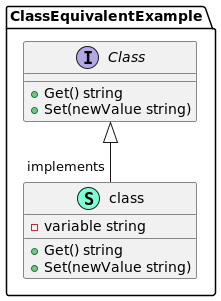
\includegraphics{part/memoria_descriptiva/ClassEquivalentInGolang}

por qué es importante concebir esta estructura:

\begin{itemize}
    \item Evitamos la instanciación no consistente, lo cual solo se garantiza a traves del método si exportado NewClass
    \item evitamos accesos no deseados al seteo de variables. Si las pusieramos publicas seria posible.
\end{itemize}

como contrapartida tenemos que escribir más codigo. poniendo como comparación una clase java o C++ no podemos decir que en cantidad de lineas escritas se aumente o disminuya. En cuestión de conceptos aprendidos en Golang sólamente trabaja con interfaces y structs contra el concepto de clase y herencia.

\subsubsection{Capas}

Conceptualmente el estará concebido en capas. Las capas cuanto más profundas sean menos tenderán a cambiar, seran las bases del proyecto y de lo que depende todo lo demas. si hay cambios en las capas superiores no afectaran al interior. Si hay cambios en el interior afectarán a todo, es por esto que el diseño del interior se concibe como Dominio de la aplicación llamado DDD.

en el proceso iterativo del desarrollo hay partes que van quedando más rígidas al estar más definidas. Todo se acopla a ello eso es el dominio. Es por esto que cuando empiezas a desarrollar conceptos nuevos puede ser necesario implementarlo en aplicación mientras se va viendo claro y luego refactorizar para incluirlo en el dominio una vez está claro.
Veamos un ejemplo:

\begin{figure}
    
\dirtree{%
    .1 Project .
        .2 Adapter.
            .3 in.
                .4 Http.
                .4 GRPC.
            .3 out.
                .4 Mysql.
                .4 GRPC.
        .2 Application.
            .3 Port.
                .4 in.
                    .5 <Domain Concept>.
                        .6 UseCase.
                            .7 SomeCommands.
                                .8 Command.
                                .8 CommandUseCase.
                            .7 SomeQuery.
                                .8 Query.
                                .8 QueryUseCase.
                            .7 SomeEventHandler.
                                .8 Event.
                                .8 EventUseCase.
                .4 out.
                    .5 External out interactions.
        .2 Domain.
            .3 EntityName.
}\label{directoryStructure}
    \caption{}
    \label{fig:ProjectfolderStructure}
\end{figure}

En realidad toda estructura es para que visualmente se entienda como está concebido el proyecto. nuestro objetivo siempre tiene que ser que no haya imports (dependencias) de paquetes de fuera hacia adentro


para entender mejor el objetivo de estas capas podemos entenderlas de forma más simple como lo que lo que hay más en la superficie es lo que más grado de incertidumbre tiene, es decir, lo que más expuesto al cambio está. por lo tanto queremos separarlo lo máximo posible del código que si está cerrado al cambio y abierto sólo a la extensión. No hay que confundirlo tanto con el principio OpenClose que siempre se aplica en toda la aplicación si no como lo que es susceptible de quedar como codigo muerto, inservible, con mala sintaxis debido al desconocimiento de librerias.

Por orden sabemos que la capa de adapter donde vamos a investigar acerca de GRPC, donde no sabemos ni la librería que vamos a utilizar, Mysql donde tenemos que escoger un paquete de ORM entre todos los disponibles en el mercado opensource. Es seguro que habrá elecciones de estas herramientas que después de estudiadas no respondan a nuestras espectativas y quede como linea futura su sustitución. Este es el devenir inevitable y típico de un software, para no deshechar partes del código que sí sean reutilizables o estén completamente terminadas nos desacoplamos de estos puntos calientes. Más aún siendo un proyecto con un tiempo muy limitado y queriendo despejar dudas en muchos frentes com prioridad versus a la perfección se va a optar en muchas ocasiones por dejar código funcional sin ninguna atención a la calidad, esto ocurre en todos los proyecctos con deadlines ajustados. Esta filosofia nos proteje y ayuda a usar la rapidez sin sacrificar la estabilidad y dejando la suciedad sólo en los puntos que no son críticos.


Un punto interesante de esta estructura son los Application port out. En qu'e se diferencia del recorder de dominio por ejemplo que es una interfaz de un adaptador de salida a base de datos. Pongamos por ejemplo que cuando se crea una Entity hay un concepto core de dominio que sea lanzar un evento entityNameCreated. No queremos bajo ningún concepto que la lógica de crear la Entity y que se lance el evento quepa la posibilidiad de ejecutarse por separado o de ejecutarse una pero no otra. Es por esto que está dentro de dominio y para ello crearemos un Recorder service que haga uso del Recorder y esté junto la creacion y el lanzamiento del evento. Haciendo el recorder interface privado y solo exponiendo el RecorderService de tal forma que no se pueda usar por separado.

Ahora imaginemos que tenemos el siguiente caso de uso:
Cada vez que se crea una Entity mediante GRPC queremos puntualmente que si la entity Tiene un campo name este sea \textit{ejemplo} entonces se envíe un correo electrónico avisando a administración de que se ha creado una entity con dicho name.
pero si se crea mediante terminal significa que lo está haciendo la propia administración y por tanto el correo no es necesario. Si en el Dominio Recorder implementamos la lógica de enviar siempre el correo no podríamos evitarlo, además de que no es un concepto de consistencia de dominio. si no se enviara el correo los datos son validos. si quisieramos meterlo en dominio tendríamos que enviar la información de quién lo está creado para saber si mandar el correo o no haciéndo la lógica más compleja y difusa por algo que en realidad no trata de la consistencia de la aplicación si no de un caso de uso en concreto. En este caso creariamos un Port.Out.Email.EmailSenderOnCreation(name) y lo implementariamos en los adaptadores de salida donde configuraríamos el correo de administración. este puerto de salida sería utilizado en el puerto de entrada de grpc Create

\begin{figure}
    
\dirtree{%
    .1 Project .
        .2 Adapter.
            .3 in.
                .4 GRPC.
                    .5 CreateEntityGrpcCall.
                .4 Console.
                    .5 CreateEntityTerminalCommand.
            .3 out.
                .4 Email.
                    .5 SendEmailOnCreationImplementation (*1).
                .4 Mysql.
                    .5 SaveEntityImplementation (*2).
        .2 Application.
            .3 Port.
                .4 in.
                    .5 Entity.
                        .6 CreateUseCase.
                            .7 CreateCommand.
                                .8 CreateCommand (using sendEmail param in this example).
                                .8 CreateUseCase.
                            .7 SomeEventHandler.
                                .8 CreationEvent.
                                .8 CreationEventUseCase.
                .4 out.
                    .5 Email.
                        .6 SendEmailConCreation (interface for *1).
        .2 Domain.
            .3 Entity.
                .4 EntityName.go.
                .4 RecorderService.go (using Recorder.go and ensuring to raise CreationEvent together with the recording).
                .4 recorder.go (interface for *2).
}\label{directoryStructureOut}
    \caption{}
    \label{fig:ProjectfolderStructurePortOut}
\end{figure}

